\documentclass{beamer}

\title{Application of Bayesian methods to modelling of extreme precipitation events}
\author{\sffamily Kári Hlynsson}
\institute{\sffamily University of Iceland}
\date{\sffamily January 2025}

\logo{\includegraphics[height=1.15cm]{{../img/hi_logo.pdf}}\hspace{0.25cm}}
\setbeamertemplate{navigation symbols}{}
\usetheme{Singapore}

\setbeamertemplate{title page}[default][left]
\setbeamertemplate{frametitle}[default][left]

\usepackage{xcolor}
\usepackage{graphicx}
\usepackage{tikz}
\usetikzlibrary{arrows}
\usetikzlibrary{arrows.meta,bending,positioning}

\usepackage{booktabs}

\graphicspath{{img}}

\definecolor{islrred}{HTML}{990000}
\definecolor{islrgreen}{HTML}{009900}
\definecolor{islrblue}{HTML}{3333b3}
\let\OldTexttt\texttt
\renewcommand{\texttt}[1]{\OldTexttt{{\textcolor{islrred}{#1}}}}

\let\OldTextit\textit
\renewcommand{\textit}[1]{\OldTextit{{\textcolor{islrgreen}{#1}}}}

% Ensure Times New Roman for math
\usepackage{amsmath, amsfonts, amssymb}
\usefonttheme[onlymath]{serif}
\usepackage{inter}
\usepackage{newtx}

\graphicspath{{../img}}

\begin{document}

\begin{frame}
  \titlepage 
\end{frame}

\begin{frame}{Introduction \footnotesize (1/2)}
  \begin{itemize}
    \setlength{\itemsep}{0.75em}
    \item Oct. 29, 2024: \(\approx 400\) mm of rain (\(\approx 1\) year's worth)
      fell in 8 hours across Valencia, Castilla-La Mancha, and Andalusia, Spain.

    \item Casualties: 232 dead, 3 missing.

    \item Damages: \(\approx\) \texteuro \(1\) billion to housing and infrastructure.

    \item Modelling \textit{extreme precipitation events} vital in mitigating
      damage to infrastructure and human life, and elucidating links to
      warming climate
  \end{itemize}
\end{frame}

\begin{frame}{Introduction \footnotesize (2/2)}
  \textbf{\sffamily Fisher-Tippett theorem.}

    If \((X_n)_{n \in \mathbf N}\) are i.i.d., \(M_n := \max\{X_1, \ldots,
    X_n\}\), and there exist normalising sequences \(a_n \in \mathbf{R}_+\)
    and \(b_n \in \mathbf{R}\) such that
    \[
      \lim_{n \to \infty} \Pr\left\{\frac{M_n - b_n}{a_n} \leq y\right\}
      \to G(y),
    \]
    then necessarily \(G(y) = \mathrm{GEV}(y \mid \mu, \sigma, \xi)\), where
    \[
      \mathrm{GEV}(y \mid \mu, \sigma, \xi)
      = \begin{cases}
          \exp\left(-\big[1 + \xi (y - \mu)/\sigma\big]^
          {-1/\xi}_+\right), &\xi \neq 0, \\
          \exp\left(-\exp\left[-(y - \mu)/\sigma\right]
          \right), &\xi = 0.
      \end{cases}
    \]
\end{frame}

\begin{frame}{Overview}
  \begin{itemize}
    \setlength{\itemsep}{0.75em}
    \item Bayesian modelling framework 
    \item Model selection and evaluation
    \item Results and discussion
  \end{itemize}
\end{frame}

\begin{frame}{The data \footnotesize (1/2)}
  \begin{itemize}
    \setlength{\itemsep}{0.75em}
    \item Raw data from Southern England spans \(\approx 132\) years of daily
      cumulative precipitation measurements in millimetres over 24 hour period.

    \item Aggregated into annual block maxima
      \[
        y_t = \max\{X_1^{(t)}, \ldots, X_{365}^{(t)}\},
      \]
      where \(X_1^{(t)}, \ldots, X_{365}^{(t)}\) are daily measurements from
      year \(t\).

    \item Result is a data set numbering \(n = 132\) measurements.

    \item Interested in modelling \textit{extreme values} in \(y = (y_1,
      \ldots, y_n)\).
  \end{itemize}
\end{frame}

\begin{frame}{The data \footnotesize (2/2)}
  \begin{figure}
    \centering
    \includegraphics[width=\textwidth]{trendplot.pdf}
  \end{figure}
\end{frame}

\begin{frame}{Modelling framework}
  \begin{itemize}
    \setlength{\itemsep}{0.75em}
    \item Response layer \(y\) is assigned generalised extreme value (GEV)
      distribution

    \item Compare \textit{stationary} models with fixed parameters and
      \textit{non-stationary} models with evolving location parameter over
      time, \(\mu_t\). Does a time trend improve model fit?

    \item MCMC applied to sample posterior \(\pi(\theta \mid y)\). 1000 samples
      for burn-in, 8000 for sampling. Convergence estimated by trace plots,
      ACF, and \(\hat R\).

    \item LOOIC / WAIC and PPC for model selection and evaluation
  \end{itemize}
\end{frame}

\begin{frame}{Stationary model}
  \begin{itemize}
    \setlength{\itemsep}{0.75em}
    \item Response layer: \(y \sim \mathrm{GEV}(\mu, \sigma, \xi)\)

    \item Latent layer: \(\mu \sim \mathrm N(0, \sigma_\mu)\),
      \(\sigma \sim \mathrm{Exp}(\lambda_\sigma)\), \(\xi \sim \mathrm{Beta}
      (\alpha_\xi, \beta_\xi)\) on interval \((-0.5, 0.5)\).

    \item \(\sigma_\mu = 10\), \(\lambda_\sigma = 3\), \(\alpha_\xi = \beta_\xi = 4\)
  \end{itemize}

  \begin{figure}[H]
      \centering
      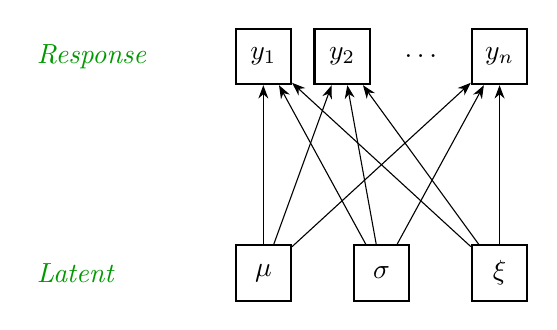
\begin{tikzpicture}
      \node[anchor = west] at (-3, 0) {\textit{Response}};
      \node[anchor = west] at (-3, -2.75) {\textit{Latent}};
      \begin{scope}[every node/.style={rectangle, minimum size = 20, thick,draw}]
          \node (D1) at (0,0) {\(y_1\)};
          \node (D2) at (1,0) {\(y_2\)};
          \node (D3) at (3,0) {\(y_n\)};
          \node (P1) at (0, -2.75) {\(\mu\)};
          \node (P2) at (1.5, -2.75) {\(\sigma\)};
          \node (P3) at (3, -2.75) {\(\xi\)};
      \end{scope}

      \begin{scope}[>={Stealth[black]},
                    every node/.style={fill=white,circle},
                    every edge/.style={draw}]
          \path [->] (P1) edge (D1);
          \path [->] (P1) edge (D2);
          \path [->] (P1) edge (D3);
          \path [->] (P2) edge (D1);
          \path [->] (P2) edge (D2);
          \path [->] (P2) edge (D3);
          \path [->] (P3) edge (D1);
          \path [->] (P3) edge (D2);
          \path [->] (P3) edge (D3);
      \end{scope}
      \node at (2,0) {\(\ldots\)};
      \end{tikzpicture}
    \end{figure}
\end{frame}

\begin{frame}{Non-stationary model (linear time trend)}
  \begin{itemize}
    \setlength{\itemsep}{0.75em}
    \item Response layer: \(y_t \sim \mathrm{GEV}(\mu_t, \sigma, \xi)\)

    \item Latent layer: \(\mu_t = \mu_0 (1 + \Delta(t - t_c))\),
      \(\sigma \sim \mathrm{Exp}(\lambda_\sigma)\), \(\xi \sim \mathrm{Beta}(\alpha_\xi,
      \beta_\xi)\) on \((-0.5, 0.5)\)

    \item Hyperparameter layer: \(\mu_0 \sim \mathrm{N}(0, \sigma_{\mu_0})\),
      \(\Delta \sim \mathrm N (0, \sigma_\Delta)\), where \(\sigma_{\mu_0} =
      \sigma_\Delta = 10\), \(t_c = \lfloor N/2 \rfloor\) 
  \end{itemize}

  \begin{figure}[H]
      \centering
      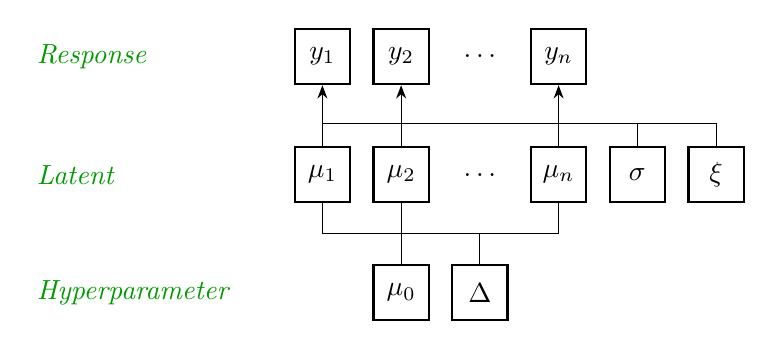
\begin{tikzpicture}
      \node[anchor = west] at (-3.75, 0) {\textit{Response}};
      \node[anchor = west] at (-3.75, -1.5) {\textit{Latent}};
      \node[anchor = west] at (-3.75, -3) {\textit{Hyperparameter}};

      \begin{scope}[every node/.style={rectangle, minimum size = 20, thick,draw}]
          \node (D1) at (0,0) {\(y_1\)};
          \node (D2) at (1,0) {\(y_2\)};
          \node (D3) at (3,0) {\(y_n\)};
          \node (P1) at (0,-1.5) {\(\mu_1\)};
          \node (P2) at (1,-1.5) {\(\mu_2\)};
          \node (P3) at (3,-1.5) {\(\mu_n\)};
          \node (p3) at (4.0,-1.5) {\(\sigma\)};
          \node (p3) at (5.0,-1.5) {\(\xi\)};
          \node (p1) at (1,-3.0) {\(\mu_0\)};
          \node (p1) at (2,-3.0) {\(\Delta\)};
      \end{scope}

      \begin{scope}[>={Stealth[black]},
                    every node/.style={fill=white,circle},
                    every edge/.style={draw}]
          \path [->] (P1) edge (D1);
          \path [->] (P2) edge (D2);
          \path [->] (P3) edge (D3);
          \draw (4.0, -1.15) |- (4, -0.85);
          \draw (4, -0.85) -- (0, -0.85);
          \draw (5.0, -1.15) |- (4, -0.85);
          \draw (5, -0.85) -- (0, -0.85);
          \draw (1, -2.65) -- (1, -2.25);
          \draw (2, -2.65) -- (2, -2.25);
          \draw (1.5, -2.25) -| (P1);
          \draw (1.5, -2.25) -| (P2);
          \draw (1.5, -2.25) -| (P3);
      \end{scope}
      \node at (2,0) {$\ldots$};
      \node at (2,-1.5) {$\ldots$};
      \end{tikzpicture}
    \end{figure}
\end{frame}

\begin{frame}{Non-stationary model (piecewise time trend) \footnotesize (1/3)}
  \begin{itemize}
    \setlength{\itemsep}{0.75em}
    \item Partition \(T = \{1, \ldots, n\}\) into \(m\) equally spaced
      time points, \(1 = t_1 < \cdots < t_m < n\). The partition granularity
      \(m\) is tuned for optimal results.

    \item Response layer: \(y_t \sim \mathrm{GEV}(\mu_t, \sigma, \xi)\)

    \item Latent layer: \(\mu_t = \mu_0 + \sum_{j = 1}^m \mu_j(t)\) where 
      \(\mu_j(t) = \beta_j \mathbf 1_{\{t \geq t_j\}} (t - t_j)\).

    \item Hyperparameter layer: \(\mu_0 \sim \mathrm N(0, \sigma_{\mu_0})\),
    \(\beta_1 \sim \mathrm{N}(0, \sigma_\beta^{(1)})\) with \(\sigma_{\mu_0} = 10\),
    and \(\sigma_\beta^{(1)} = 0.10\). Three priors for remaining \(\beta_j\):
      \begin{itemize}
        \setlength{\itemsep}{0.5em}
        \item I.I.D.: \(\beta_{j + 1} \sim \mathrm{N}(0, \sigma_\beta)\)
          for \(j \geq 1\),

        \item R.W.: \(\beta_{j + 1} \sim \mathrm{N}(\beta_j, \sigma_\beta)\)
          for \(j \geq 1\),

        \item AR(1): \(\beta_{j + 1} \sim \mathrm{N}(\phi \beta_j, \sigma_\beta)\)
          for \(j \geq 1\), \(\phi \sim \mathrm{Unf}(-1, 1)\),
      \end{itemize}
      where \(\sigma_\beta = 0.01\).
  \end{itemize}
\end{frame}

\begin{frame}{Non-stationary model (piecewise time trend) \footnotesize (2/3)}
  \begin{figure}[H]
      \centering
      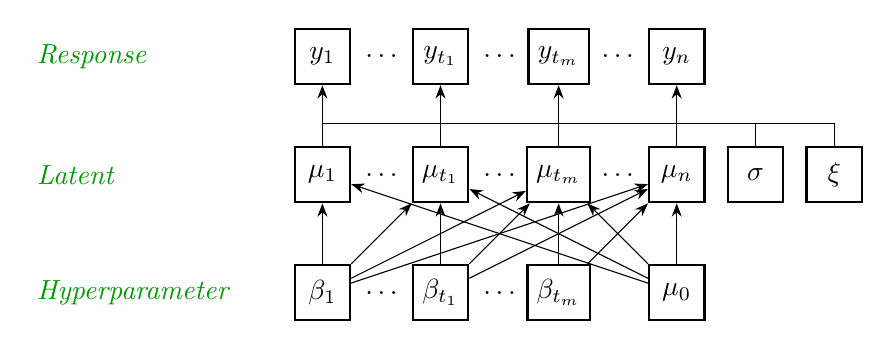
\begin{tikzpicture}
      \node[anchor = west] at (-3.75, 0) {\textit{Response}};
      \node[anchor = west] at (-3.75, -1.5) {\textit{Latent}};
      \node[anchor = west] at (-3.75, -3) {\textit{Hyperparameter}};

      \begin{scope}[every node/.style={rectangle, minimum size = 20, thick,draw}]
          \node (D1) at (0,0) {\(y_1\)};
          \node (D2) at (1.5,0) {\(y_{t_1}\)};
          \node (D3) at (3,0) {\(y_{t_{m}}\)};
          \node (D4) at (4.5,0) {\(y_{n}\)};
          \node (P1) at (0,-1.5) {\(\mu_1\)};
          \node (P2) at (1.5,-1.5) {\(\mu_{t_1}\)};
          \node (P3) at (3,-1.5) {\(\mu_{t_m}\)};
          \node (P4) at (4.5,-1.5) {\(\mu_n\)};
          \node (P5) at (5.5,-1.5) {\(\sigma\)};
          \node (P6) at (6.5,-1.5) {\(\xi\)};
          \node (p1) at (0,-3.0) {\(\beta_1\)};
          \node (p2) at (1.5,-3.0) {\(\beta_{t_1}\)};
          \node (p3) at (3,-3.0) {\(\beta_{t_m}\)};
          \node (p4) at (4.5,-3.0) {\(\mu_0\)};
      \end{scope}

      \begin{scope}[>={Stealth[black]},
                    every node/.style={fill=white,circle},
                    every edge/.style={draw}]
        \path [->] (P1) edge (D1);
        \path [->] (P2) edge (D2);
        \path [->] (P3) edge (D3);
        \path [->] (P4) edge (D4);
        \path [->] (p1) edge (P1);
        \path [->] (p1) edge (P2);
        \path [->] (p1) edge (P3);
        \path [->] (p1) edge (P4);
        \path [->] (p2) edge (P2);
        \path [->] (p2) edge (P3);
        \path [->] (p2) edge (P4);
        \path [->] (p3) edge (P3);
        \path [->] (p3) edge (P4);
        \path [->] (p4) edge (P1);
        \path [->] (p4) edge (P2);
        \path [->] (p4) edge (P3);
        \path [->] (p4) edge (P4);
        \draw (5.5, -1.15) |- (5.5, -0.85);
        \draw (6.5, -0.85) -- (0, -0.85);
        \draw (6.5, -1.15) |- (6.5, -0.85);
      \end{scope}
        \node at (0.75,0) {\(\ldots\)};
        \node at (2.25,0) {\(\ldots\)};
        \node at (3.75,0) {\(\ldots\)};
        \node at (0.75,-1.5) {\(\ldots\)};
        \node at (2.25,-1.5) {\(\ldots\)};
        \node at (3.75,-1.5) {\(\ldots\)};
        \node at (0.75,-3.0) {\(\ldots\)};
        \node at (2.25,-3.0) {\(\ldots\)};
      \end{tikzpicture}
    \end{figure}
\end{frame}

\begin{frame}{Non-stationary model (piecewise time trend) \footnotesize (3/3)}
  \begin{figure}
    \centering
    \includegraphics[width = \textwidth]{beta_basis.pdf}
  \end{figure}
\end{frame}

\begin{frame}{Model selection (1/2)}
  \begin{table}[H]
    \centering
    \footnotesize
    \begin{tabular}{rccccc}
      \toprule
      &            &                           & \multicolumn{3}{c}{Piecewise trend}     \\
                                                          \cmidrule(rl){4-6}
                   & Stationary & Linear trend & AR(1)       & I.I.D.      & R.W.        \\
      \midrule
      \(\widehat{\mathrm{LOOIC}}\) & 965.2      & 955.0        & 954.2 (6)  & 953.8 (18)   & \textbf{953.2 (18)}  \\
      \(\widehat{\mathrm{WAIC}}\)  & 961.9      & 951.9        & 951.1 (4)  & 951.0 (33)   & \textbf{950.3 (18)}  \\
      \bottomrule
    \end{tabular}
  \end{table}
\end{frame}

\begin{frame}{Model selection \footnotesize (2/2)}
  \begin{figure}[H]
    \centering
    \includegraphics[width=\textwidth]{optim_m.pdf}
  \end{figure}
\end{frame}

\begin{frame}{Model evaluation \footnotesize (1/3)}
  \begin{figure}[H]
    \centering
    \includegraphics[width = \textwidth]{ppc_edf_overlay.pdf}
  \end{figure} 
\end{frame}

\begin{frame}{Model evaluation \footnotesize (2/3)}
  \begin{figure}[H]
    \centering
    \includegraphics[width = \textwidth]{ppc_rw.pdf}
  \end{figure} 
\end{frame}

\begin{frame}{Model evaluation \footnotesize (3/3)}
  \begin{figure}[H]
    \centering
    \includegraphics[width = \textwidth]{qqplot_yrep.pdf}
  \end{figure} 
\end{frame}

\begin{frame}{Model comparison}
  \begin{figure}[H]
    \centering
    \includegraphics[width = \textwidth]{post_mean.pdf}
  \end{figure}
\end{frame}

\begin{frame}{Results and discussion}
  \begin{itemize}
    \setlength{\itemsep}{0.75em}
    \item Models involving time trend show significant increase in
      accuracy, suggesting that maximum annual precipitation is evolving
      with time

    \item Flexibility of piecewise linear trend superior to simple linear
      time trend with respect to accuracy

    \item Rising trend observed in first 100 years which wanes in the
      remaining 30 years -- hard to tell whether this is a continued trend
      as opposed to instability in extremes.

    \item Observed trend restricted to location where data are obtained --
      for a more wholistic picture, need to analyse more catchments and
      include spatial effects.
  \end{itemize} 
\end{frame}

\end{document}

